\documentclass[12pt, a4paper]{article}
\usepackage[utf8]{inputenc}
\usepackage[T1]{fontenc}
\usepackage{geometry}
\geometry{
    top=3cm,
    bottom=3cm,
    left=2.5cm,
    right=2.5cm
}
\usepackage{xcolor}
\usepackage{amsmath}  
\usepackage{amssymb}
\usepackage{listings}
\usepackage{graphicx}

\begin{document}

\begin{titlepage}
    \begin{center}
        \textbf{BABEȘ-BOLYAI UNIVERSITY CLUJ-NAPOCA} \\[0.5cm]
        \textbf{FACULTY OF MATHEMATICS AND COMPUTER SCIENCE} \\[0.5cm]
        \textbf{SPECIALIZATION MATHEMATICS-COMPUTER SCIENCE}
        
        \vspace*{6cm} 
        
        {\LARGE \textbf{DIPLOMA THESIS}} \\[2cm]
        
        {\Large \textbf{Function Interpolation}}
        
    \end{center}
    
    \vspace*{4cm} 
    
    \noindent
    \begin{minipage}[t]{0.7\textwidth}
        \textbf{Supervisor} \\[0.5cm]
        \textcolor{red}{\textbf{Dr. LŐRINCZI Ábel, Asistent Universitar}}
    \end{minipage}%
    \begin{minipage}[t]{0.3\textwidth}
        \vspace*{1.5cm} 
        \raggedleft
        \textit{Author \\ Romanică Gabriel}
    \end{minipage}
    
    \vfill
    
    \begin{center}
        \textbf{2026}
    \end{center}
\end{titlepage}

\newpage
\renewcommand{\abstractname}{Abstract}
\begin{abstract}
    The approximation of functions through polynomials is a foundational concept in numerical analysis, essential for evaluating complex functions using standard arithmetic operations. This thesis explores the mathematical theory and practical implementation of polynomial interpolation, focusing on the critical transition from equidistant to optimal node distribution. We begin by detailing the classical and barycentric forms of Lagrange interpolation, followed by Newton's method using divided and finite differences. 

The core of the paper investigates Runge's phenomenon, demonstrating how high-degree polynomial interpolation on equally spaced nodes leads to catastrophic divergence. To resolve this numerical instability, Chebyshev nodes are introduced and mathematically justified through their minimax error properties. Finally, original MATLAB simulations are presented to practically validate the theoretical claims, using Newton's divided differences to explicitly contrast the unbounded error of equidistant nodes with the convergent stability of Chebyshev nodes.
\end{abstract}

\newpage

\tableofcontents

\newpage
\section{Introduction}

The ability to approximate complex mathematical functions using simpler, computable formulas is a cornerstone of numerical analysis and scientific computing. In practice, many functions encountered in engineering, physics, and computer science cannot be evaluated exactly. Interpolation provides a robust mechanism to construct a known function---typically a polynomial---that exactly matches a discrete set of data points, allowing for highly accurate approximations of the underlying unknown function.

The primary objective of this thesis is to explore the theoretical foundations of polynomial interpolation, examine its inherent numerical limitations, and demonstrate the optimal methods for achieving stable approximations. The paper is structured to guide the reader from classical definitions to practical computational implementations.

Chapter 2 introduces Lagrange interpolation, covering both its classical theoretical form and the highly efficient barycentric formulation. Chapter 3 transitions to Newton's method, detailing divided differences and the forward and backward finite difference formulas, which offer significant computational advantages when adding new data points. 

Chapter 4 highlights a fundamental limitation in numerical approximation known as Runge's phenomenon, illustrating how increasing the degree of an interpolating polynomial on equidistant nodes paradoxically leads to massive divergence and error accumulation, particularly near the boundaries of an interval. Chapter 5 introduces the mathematical cure to this problem: Chebyshev nodes. By utilizing the roots of Chebyshev polynomials, we demonstrate how the interpolation error is minimized, ensuring convergence.

Finally, Chapter 6 presents practical applications. Using custom MATLAB implementations of the interpolation algorithms, we perform numerical simulations that explicitly compare the error rates of equidistant nodes against Chebyshev nodes, proving the theoretical claims discussed in the preceding chapters.


\newpage
\section{Lagrange Interpolation}

Approximation of functions is one of the most important tasks in Numerical Analysis. Most functions encountered in mathematical problems and applications cannot be evaluated exactly, even though we usually handle them as if they were completely known quantities \cite{course4}. Interpolation provides a method to find a computable function---usually a polynomial---whose graph goes through a given set of data points.

\subsection{Classical Lagrange Form}

Given $n+1$ distinct points, called \textit{nodes}, $x_i \in [a,b]$ for $i = 0, \dots, n$, and the values $f(x_i) = y_i$ of an unknown function $f: [a,b] \rightarrow \mathbb{R}$, the goal is to find a polynomial $P(x)$ of minimum degree that satisfies the interpolation conditions:
\begin{equation}
    P(x_i) = f(x_i), \quad i = 0, \dots, n
\end{equation}

\vspace{0.5cm}
\noindent \textbf{Theorem 2.1 (Existence and Uniqueness).} \textit{There is a unique polynomial $L_n f$ of degree at most $n$, satisfying the interpolation conditions. This polynomial can be written as:}
\begin{equation}
    L_n f(x) = \sum_{i=0}^n l_i(x) f(x_i)
\end{equation}
\textit{where $l_i(x)$ are the Lagrange fundamental (basis) polynomials, defined as:}
\begin{equation}
    l_i(x) = \prod_{\substack{j=0 \\ j \neq i}}^n \frac{x - x_j}{x_i - x_j}
\end{equation}

\vspace{0.5cm}
\noindent \textbf{Example: Linear Interpolation.} Consider two distinct nodes $(x_0, y_0)$ and $(x_1, y_1)$. The polynomial of degree 1 that interpolates this data is:
\begin{equation}
    P_1(x) = \frac{x - x_1}{x_0 - x_1} y_0 + \frac{x - x_0}{x_1 - x_0} y_1
\end{equation}
For instance, to interpolate $f(x) = \sqrt{x}$ at nodes $x_0 = 1$ and $x_1 = 4$, substituting the values yields $P_1(x) = \frac{1}{3}x + \frac{2}{3}$.

While the polynomial matches the function exactly at the interpolation nodes, an error exists at all other points within the interval.

\vspace{0.5cm}
\noindent \textbf{Theorem 2.2 (Interpolation Error).} \textit{Let $f \in C^{n+1}[a,b]$ and consider the distinct nodes $x_0, \dots, x_n \in [a,b]$. Then there exists a $\xi \in (a,b)$ such that the interpolation remainder is:}
\begin{equation}
    (R_n f)(x) = f(x) - (L_n f)(x) = \frac{u(x)}{(n+1)!} f^{(n+1)}(\xi)
\end{equation}
\textit{where $u(x) = (x - x_0)(x - x_1) \dots (x - x_n)$.}

\subsection{Barycentric Interpolation}

The classical Lagrange formula is highly useful for theoretical proofs, but it is less desirable for practical computations \cite{course4}. Evaluating it requires $\mathcal{O}(n^2)$ floating-point operations for every value of $x$, and adding a new node requires restarting the calculation from scratch.

To improve computational efficiency, we introduce \textit{barycentric weights}:
\begin{equation}
    w_i = \frac{1}{\prod_{\substack{j=0 \\ j \neq i}}^n (x_i - x_j)}, \quad i = 0, 1, \dots, n
\end{equation}

Using these weights, the polynomial can be expressed in the \textbf{First Barycentric Formula}:
\begin{equation}
    L_n f(x) = u(x) \sum_{i=0}^n \frac{w_i}{x - x_i} f_i
\end{equation}
Once the weights are computed, evaluating $L_n f(x)$ requires only $\mathcal{O}(n)$ operations, and adding a new node updates the weights efficiently.

Furthermore, by applying the principle that the Lagrange polynomial for the constant function $f(x) \equiv 1$ is exactly $1$, we obtain the \textbf{Second Barycentric Formula}:
\begin{equation}
    L_n f(x) = \frac{\sum_{i=0}^n \frac{w_i}{x - x_i} f_i}{\sum_{i=0}^n \frac{w_i}{x - x_i}}
\end{equation}
This formula is highly advantageous because any common factors within the weights $w_i$ can be canceled without altering the final polynomial evaluation \cite{course4}.
\vspace{0.5cm}

\noindent \textbf{Example: Second Barycentric Formula by Hand.}
Let us interpolate the function $f(x) = x^2$ using three nodes: $x_0 = 0, x_1 = 1, x_2 = 2$. The corresponding function values are $f_0 = 0, f_1 = 1, f_2 = 4$. We want to evaluate the polynomial at $x = 1.5$.

First, we calculate the barycentric weights $w_i = \prod_{j \neq i} (x_i - x_j)^{-1}$:
\begin{align*}
    w_0 &= \frac{1}{(0 - 1)(0 - 2)} = \frac{1}{2} \\
    w_1 &= \frac{1}{(1 - 0)(1 - 2)} = -1 \\
    w_2 &= \frac{1}{(2 - 0)(2 - 1)} = \frac{1}{2}
\end{align*}

Next, we compute the terms $\frac{w_i}{x - x_i}$ for $x = 1.5$:
\begin{align*}
    i=0&: \quad \frac{1/2}{1.5 - 0} = \frac{1}{3} \\
    i=1&: \quad \frac{-1}{1.5 - 1} = -2 \\
    i=2&: \quad \frac{1/2}{1.5 - 2} = -1
\end{align*}

Finally, we apply the Second Barycentric Formula:
\begin{equation}
    L_2(1.5) = \frac{\sum \frac{w_i}{x - x_i} f_i}{\sum \frac{w_i}{x - x_i}} = \frac{\frac{1}{3}(0) + (-2)(1) + (-1)(4)}{\frac{1}{3} - 2 - 1} = \frac{-6}{-8/3} = 2.25
\end{equation}
This perfectly matches the exact function evaluation $f(1.5) = 1.5^2 = 2.25$.
\subsection{Implementation Notes}

When implementing the Second Barycentric Formula programmatically (e.g., in MATLAB), a critical edge case must be managed. The interpolation polynomial is undefined when $x$ exactly matches one of the nodes $x_i$, due to a division by zero in both the numerator and denominator \cite{course4}. 

Mathematically, the limit as $x \to x_i$ is exactly $f(x_i)$. Therefore, a robust implementation must explicitly check if $x$ is equivalent to a node $x_i$ (within machine precision tolerance) and immediately return the corresponding function value $f(x_i)$ to ensure continuous extension.

\newpage
\section{Newton Interpolation}

While the Lagrange form elegantly proves the existence and uniqueness of the interpolation polynomial, it has a significant computational drawback: if a new data point is added, the entire polynomial must be recalculated from scratch \cite{course5, runge}. Newton's interpolation method resolves this by expressing the polynomial in a hierarchical form, where adding a new node simply requires adding a new term to the existing polynomial without altering the previously calculated coefficients.

\subsection{Divided Differences}

Newton's interpolation polynomial relies on the concept of \textit{divided differences}. Given $n+1$ pairs of points $(x_k, y_k)$ for $k = 0, \dots, n$, the divided differences are defined recursively as follows \cite{runge}:

\begin{itemize}
    \item \textbf{Zeroth-order:} $f[x_k] = f(x_k) = y_k$
    \item \textbf{First-order:} $f[x_k, x_{k+1}] = \frac{f[x_{k+1}] - f[x_k]}{x_{k+1} - x_k}$
    \item \textbf{i-th order:} $f[x_k, x_{k+1}, \dots, x_{k+i}] = \frac{f[x_{k+1}, \dots, x_{k+i}] - f[x_k, \dots, x_{k+i-1}]}{x_{k+i} - x_k}$
\end{itemize}

Using these coefficients, Newton's interpolation polynomial $N_n f(x)$ of degree at most $n$ is written as \cite{course5, runge}:
\begin{equation}
    N_n f(x) = f[x_0] + \sum_{i=1}^n f[x_0, \dots, x_i] \prod_{j=0}^{i-1} (x - x_j)
\end{equation}

By the uniqueness of the interpolation polynomial, $N_n f(x)$ is mathematically equivalent to the Lagrange polynomial $L_n f(x)$ for the same set of nodes, merely expressed in a different algebraic form \cite{course5}.

\vspace{0.5cm}
\noindent \textbf{Theorem 3.1 (Interpolation Error for Newton's Form).} \textit{The remainder (error) of the Newton interpolation polynomial is given by:}
\begin{equation}
    R_n f(x) = \frac{f^{(n+1)}(\xi)}{(n+1)!} (x - x_0)(x - x_1) \dots (x - x_n)
\end{equation}
\textit{where $\xi$ lies in the smallest interval containing the nodes $x_0, \dots, x_n$ and the point $x$ \cite{course5}.}

\vspace{0.5cm}
\noindent \textbf{Example: Divided Differences by Hand.}
Let us interpolate $f(x) = x^3$ at the nodes $x_0 = 0, x_1 = 1, x_2 = 2, x_3 = 3$. The function values are $0, 1, 8, 27$. We construct the divided difference table:

\begin{center}
\begin{tabular}{c|c|ccc}
$x_k$ & $f[x_k]$ & 1st Order & 2nd Order & 3rd Order \\
\hline
0 & 0  &                 &                 & \\
  &    & $\frac{1-0}{1-0}=1$ &                 & \\
1 & 1  &                 & $\frac{7-1}{2-0}=3$ & \\
  &    & $\frac{8-1}{2-1}=7$ &                 & $\frac{6-3}{3-0}=1$ \\
2 & 8  &                 & $\frac{19-7}{3-1}=6$ & \\
  &    & $\frac{27-8}{3-2}=19$ &               & \\
3 & 27 &                 &                 & \\
\end{tabular}
\end{center}

The coefficients for Newton's polynomial are the top edge of the table: $D_0=0, D_1=1, D_2=3, D_3=1$. The polynomial is:
\begin{equation}
    N_3(x) = 0 + 1(x-0) + 3(x-0)(x-1) + 1(x-0)(x-1)(x-2)
\end{equation}
Evaluating at $x = 1.5$ yields $1.5 + 3(1.5)(0.5) + (1.5)(0.5)(-0.5) = 1.5 + 2.25 - 0.375 = 3.375$, matching $1.5^3 = 3.375$.

\subsection{Forward and Backward Differences}

When the interpolation nodes are equally spaced (equidistant), such that $x_i = x_0 + ih$ for a constant step size $h$, computing divided differences becomes unnecessary. Instead, the polynomial can be constructed using simpler finite differences \cite{course5}.

\textbf{Newton's Forward Difference Formula} uses the forward difference operator $\Delta^k f_i = \Delta^{k-1} f_{i+1} - \Delta^{k-1} f_i$. By substituting $s = \frac{x - x_0}{h}$, the polynomial takes the form \cite{course5}:
\begin{equation}
    L_n f(x) = f_0 + \binom{s}{1}\Delta f_0 + \binom{s}{2}\Delta^2 f_0 + \dots + \binom{s}{n}\Delta^n f_0
\end{equation}
This formula yields the highest precision when evaluating the polynomial near the beginning of the dataset (close to $x_0$) \cite{course5}.

\textbf{Newton's Backward Difference Formula} uses the backward difference operator $\nabla^k f_i = \nabla^{k-1} f_i - \nabla^{k-1} f_{i-1}$. Using the substitution $t = \frac{x - x_n}{h}$, the polynomial is written as \cite{course5}:
\begin{equation}
    L_n f(x) = f_n + \frac{t}{1!}\nabla f_n + \frac{t(t+1)}{2!}\nabla^2 f_n + \dots + \frac{t(t+1)\dots(t+n-1)}{n!}\nabla^n f_n
\end{equation}
Conversely, the backward formula is preferred when evaluating points near the end of the dataset (close to $x_n$) \cite{course5}.

\vspace{0.5cm}
\noindent \textbf{Example: Forward Differences by Hand.}
Using the same function $f(x) = x^3$ and equidistant nodes $x_0=0, x_1=1, x_2=2, x_3=3$, the step size is $h=1$. The forward differences are:
\begin{itemize}
    \item $\Delta^0 f = [0, 1, 8, 27]$
    \item $\Delta^1 f = [1, 7, 19]$
    \item $\Delta^2 f = [6, 12]$
    \item $\Delta^3 f = [6]$
\end{itemize}

To evaluate the polynomial at $x = 1.5$, we calculate the parameter $s = \frac{x - x_0}{h} = \frac{1.5 - 0}{1} = 1.5$. Using the forward coefficients $\Delta^k f_0$ (the first element of each difference array):
\begin{equation}
    P(1.5) = 0 + 1.5(1) + \frac{1.5(1.5-1)}{2}(6) + \frac{1.5(1.5-1)(1.5-2)}{6}(6)
\end{equation}
Simplifying the terms yields $1.5 + 2.25 - 0.375 = 3.375$, confirming the consistency of the methods.

\subsection{Implementation Notes}

From a software implementation perspective (e.g., in MATLAB), generating Newton's polynomial involves a two-step process. 

First, the divided differences are computed and stored. This is typically done using a lower triangular matrix or a 1D array updated in-place to save memory, requiring $\mathcal{O}(n^2)$ operations. The diagonal of this conceptual matrix provides the coefficients $D_i = f[x_0, \dots, x_i]$ \cite{course5}.

Second, the polynomial is evaluated at a given point $x$. To avoid redundant multiplications and reduce the evaluation cost to $\mathcal{O}(n)$ operations, the polynomial must be evaluated using a nested multiplication structure (Horner's-like scheme) \cite{course5}:
\begin{equation}
    N_n f(x) = D_0 + (x - x_0)\left[D_1 + (x - x_1)\left[D_2 + \dots + (x - x_{n-1})D_n\right]\right]
\end{equation}
This nested form ensures computational efficiency and minimizes floating-point rounding errors during execution.

\newpage
\section{Runge's Phenomenon}

In the context of polynomial interpolation, it is natural to assume that increasing the number of interpolation nodes---and consequently the degree of the interpolating polynomial---will yield a more accurate approximation of the underlying function. However, this intuitive assumption is false for certain functions, particularly when using equidistant nodes. This counterintuitive behavior is known as \textit{Runge's phenomenon} \cite{runge}.

\subsection{The Runge Function}

The phenomenon was discovered by the German mathematician Carl David Tolmé Runge in 1901 when he was investigating the polynomial interpolation of the function:
\begin{equation}
    f(x) = \frac{1}{1 + 25x^2}
\end{equation}
evaluated on the interval $[-1, 1]$. This specific mathematical expression is now commonly referred to as the \textit{Runge function} \cite{runge}.

\subsection{Behavior with Equidistant Nodes}

When interpolating the Runge function using a polynomial $P_n(x)$ of degree $n$ over a set of $n+1$ equidistant nodes, the polynomial perfectly matches the function at the given data points. However, between the nodes---especially near the boundaries of the interval, at $x = -1$ and $x = 1$---the polynomial exhibits severe and wild oscillations \cite{runge, knorrenschild}.

As the number of nodes $n$ increases, rather than the polynomial converging closer to the true function $f(x)$, the magnitude of these oscillations grows unboundedly. Mathematically, the maximum error approaches infinity:
\begin{equation}
    \lim_{n \to \infty} \left( \max_{-1 \le x \le 1} |f(x) - P_n(x)| \right) = \infty
\end{equation}

This divergent behavior demonstrates that high-degree polynomial interpolation on equally spaced points is numerically unstable and generally unsuitable for practical approximation over wide intervals.

\subsection{The Cause of the Phenomenon}

The root cause of Runge's phenomenon lies in the behavior of the interpolation error term. Recall from Theorem 2.2 that the interpolation error is proportional to the nodal polynomial $u(x) = \prod_{i=0}^n (x - x_i)$ and the $(n+1)$-th derivative of the function.

For equidistant nodes, the amplitude of the nodal polynomial $u(x)$ becomes exceedingly large near the edges of the interval as $n$ grows. Furthermore, the higher-order derivatives of the Runge function grow rapidly \cite{runge}. The combination of these two factors causes the error term to explode near the boundaries, completely overshadowing the convergence achieved in the center of the interval.

To mitigate this catastrophic numerical instability, one must abandon equidistant nodes and select a different mathematical distribution of points that minimizes the maximum value of $u(x)$ across the entire interval.

\newpage
\section{Chebyshev Nodes}

As demonstrated by Runge's phenomenon, polynomial interpolation on equally spaced nodes can lead to catastrophic divergence near the boundaries of the interval. To guarantee convergence and minimize the maximum interpolation error, the nodes must be clustered more densely near the endpoints than in the middle. The most mathematically sound and widely used distribution for this purpose is the set of \textit{Chebyshev nodes} \cite{runge, knorrenschild}.

\subsection{Chebyshev Polynomials}

The foundation of these nodes lies in the Chebyshev polynomials of the first kind, denoted as $T_n(x)$. For $x \in [-1, 1]$, they are defined by the trigonometric relation:
\begin{equation}
    T_n(x) = \cos(n \arccos x), \quad n = 0, 1, 2, \dots
\end{equation}

These polynomials exhibit a remarkable "minimax" property: out of all monic polynomials of degree $n$, the corresponding Chebyshev polynomial has the smallest maximum absolute value on the interval $[-1, 1]$.

\subsection{Chebyshev Nodes of the First Kind}

The Chebyshev nodes are defined as the roots of the Chebyshev polynomial $T_{n+1}(x)$. For an interpolation polynomial of degree $n$, there are $n+1$ roots on the standard interval $[-1, 1]$, given by the formula \cite{runge}:
\begin{equation}
    x_k = \cos\left(\frac{2k+1}{2n+2}\pi\right), \quad k = 0, 1, \dots, n
\end{equation}
Geometrically, these points correspond to the $x$-coordinates of $n+1$ equally spaced points placed along the upper half of the unit circle.

When interpolating a function defined on an arbitrary interval $[a, b]$, these nodes cannot be used directly. They must be mapped from $[-1, 1]$ to $[a, b]$ using an affine transformation \cite{runge}:
\begin{equation}
    x_k^{[a,b]} = \frac{a+b}{2} + \frac{b-a}{2} \cos\left(\frac{2k+1}{2n+2}\pi\right)
\end{equation}

\subsection{Minimizing the Interpolation Error}

The primary advantage of Chebyshev nodes is their direct impact on the interpolation error term. Recall from Theorem 2.2 that the error depends heavily on the nodal polynomial $u(x) = \prod_{i=0}^n (x - x_i)$. 

When the interpolation nodes $x_i$ are chosen to be the Chebyshev nodes, the maximum amplitude of $u(x)$ over the interval is optimally minimized.

\vspace{0.5cm}
\noindent \textbf{Theorem 5.1 (Minimax Property of Chebyshev Nodes).} \textit{If $x_0, \dots, x_n$ are the roots of the Chebyshev polynomial $T_{n+1}(x)$, then:}
\begin{equation}
    \max_{-1 \le x \le 1} \left| \prod_{i=0}^n (x - x_i) \right| = \frac{1}{2^n}
\end{equation}

By replacing equidistant nodes with Chebyshev nodes, the amplitude of $u(x)$ is bounded and significantly reduced. This effectively eliminates the explosive oscillations near the boundaries, thus acting as the standard cure for Runge's phenomenon \cite{knorrenschild}.

\subsection{Barycentric Interpolation with Chebyshev Nodes}

Chebyshev nodes pair exceptionally well with the Second Barycentric Formula introduced in Chapter 2. When using equidistant nodes, the barycentric weights $w_j$ vary by exponentially large factors (approximately $2^n$), which amplifies floating-point rounding errors and causes instability \cite{course4}.

Conversely, when using Chebyshev points of the first kind, the weights are much more stable. After canceling common factors independent of $j$, the barycentric weights are given by \cite{course4}:
\begin{equation}
    w_j = (-1)^j \sin\left(\frac{(2j+1)\pi}{2n+2}\right), \quad j = 0, \dots, n
\end{equation}

Because these weights vary by factors of $\mathcal{O}(n)$ rather than exponentially, the barycentric evaluation remains highly stable, ensuring that small data errors near the center of the interval do not translate into massive oscillations near the edges \cite{course4}.

\newpage
\section{Applications and Numerical Simulations}

To demonstrate the theoretical concepts discussed in previous chapters, we implement the interpolation algorithms in MATLAB. The primary objective is to numerically simulate Runge's phenomenon and observe how transitioning from equidistant nodes to Chebyshev nodes minimizes the interpolation error. 

\subsection{MATLAB Implementations}

We first implement the Second Barycentric Formula for Lagrange interpolation. The algorithm computes the weights in $\mathcal{O}(n^2)$ and evaluates the polynomial using vectorized operations. Explicit handling of the singularity ($x = x_i$) is included to prevent division by zero.

\begin{lstlisting}[language=Matlab, frame=single, caption={Barycentric Lagrange Interpolation}]
function y_eval = barycentric_interp(x_nodes, y_nodes, x_eval)
    n = length(x_nodes);
    w = ones(1, n);
    % Compute barycentric weights
    for i = 1:n
        for j = 1:n
            if i ~= j
                w(i) = w(i) / (x_nodes(i) - x_nodes(j));
            end
        end
    end
    
    y_eval = zeros(size(x_eval));
    % Evaluate polynomial
    for k = 1:length(x_eval)
        exact_match = find(x_nodes == x_eval(k), 1);
        if ~isempty(exact_match)
            y_eval(k) = y_nodes(exact_match); % Handle exact node case
        else
            num = sum((w .* y_nodes) ./ (x_eval(k) - x_nodes));
            den = sum(w ./ (x_eval(k) - x_nodes));
            y_eval(k) = num / den;
        end
    end
end
\end{lstlisting}

Next, we implement Newton's method using divided differences. This algorithm computes the divided difference table (storing only the necessary diagonal to save memory) and evaluates the polynomial using nested multiplication (Horner's scheme). Per the numerical objectives of this thesis, we will strictly use this Newton formulation to compare the approximation errors in the subsequent simulations.

\begin{lstlisting}[language=Matlab, frame=single, caption={Newton Interpolation via Divided Differences}]
function y_eval = newton_div_diff(x_nodes, y_nodes, x_eval)
    n = length(x_nodes);
    D = y_nodes; % Initialize with 0th order differences
    
    % Compute divided differences in-place
    for i = 2:n
        for j = n:-1:i
            D(j) = (D(j) - D(j-1)) / (x_nodes(j) - x_nodes(j-i+1));
        end
    end
    
    y_eval = zeros(size(x_eval));
    % Evaluate using Horner's nested scheme
    for k = 1:length(x_eval)
        val = D(n);
        for i = n-1:-1:1
            val = D(i) + (x_eval(k) - x_nodes(i)) * val;
        end
        y_eval(k) = val;
    end
end
\end{lstlisting}

\subsection{Error Comparison: Equidistant vs. Chebyshev Nodes}

To visualize Runge's phenomenon, we interpolate the Runge function $f(x) = \frac{1}{1 + 25x^2}$ over the interval $[-1, 1]$. We utilize the \texttt{newton\_div\_diff} implementation and compare the maximum absolute error when using $N$ equidistant nodes versus $N$ Chebyshev nodes.

\begin{lstlisting}[language=Matlab, frame=single, caption={Simulation of Runge's Phenomenon}]
f = @(x) 1 ./ (1 + 25 * x.^2);
x_eval = linspace(-1, 1, 1000); % Dense grid for evaluation
y_exact = f(x_eval);

N_values = [5, 11, 21];

for N = N_values
    % 1. Equidistant Nodes
    x_eq = linspace(-1, 1, N);
    y_eq = f(x_eq);
    p_eq = newton_div_diff(x_eq, y_eq, x_eval);
    err_eq = max(abs(y_exact - p_eq));
    
    % 2. Chebyshev Nodes
    k = 0:N-1;
    x_cheb = cos((2*k + 1)*pi / (2*N)); 
    y_cheb = f(x_cheb);
    p_cheb = newton_div_diff(x_cheb, y_cheb, x_eval);
    err_cheb = max(abs(y_exact - p_cheb));
    
    fprintf('N = %d | Max Error (Equidistant): %.4e | Max Error (Chebyshev): %.4e\n', N, err_eq, err_cheb);
end
\end{lstlisting}

When executing the simulation, the divergence with equidistant nodes becomes immediately apparent. For $N = 11$, the maximum error is significant near the boundaries. When $N = 21$, the polynomial on equidistant nodes begins to wildly oscillate, and the numerical error explodes. Conversely, the Newton interpolation utilizing Chebyshev nodes exhibits continuous convergence; the maximum error strictly decreases as $N$ increases, successfully approximating the Runge function and validating the minimax error theory presented in Chapter 5.

\begin{figure}[h]
    \centering
    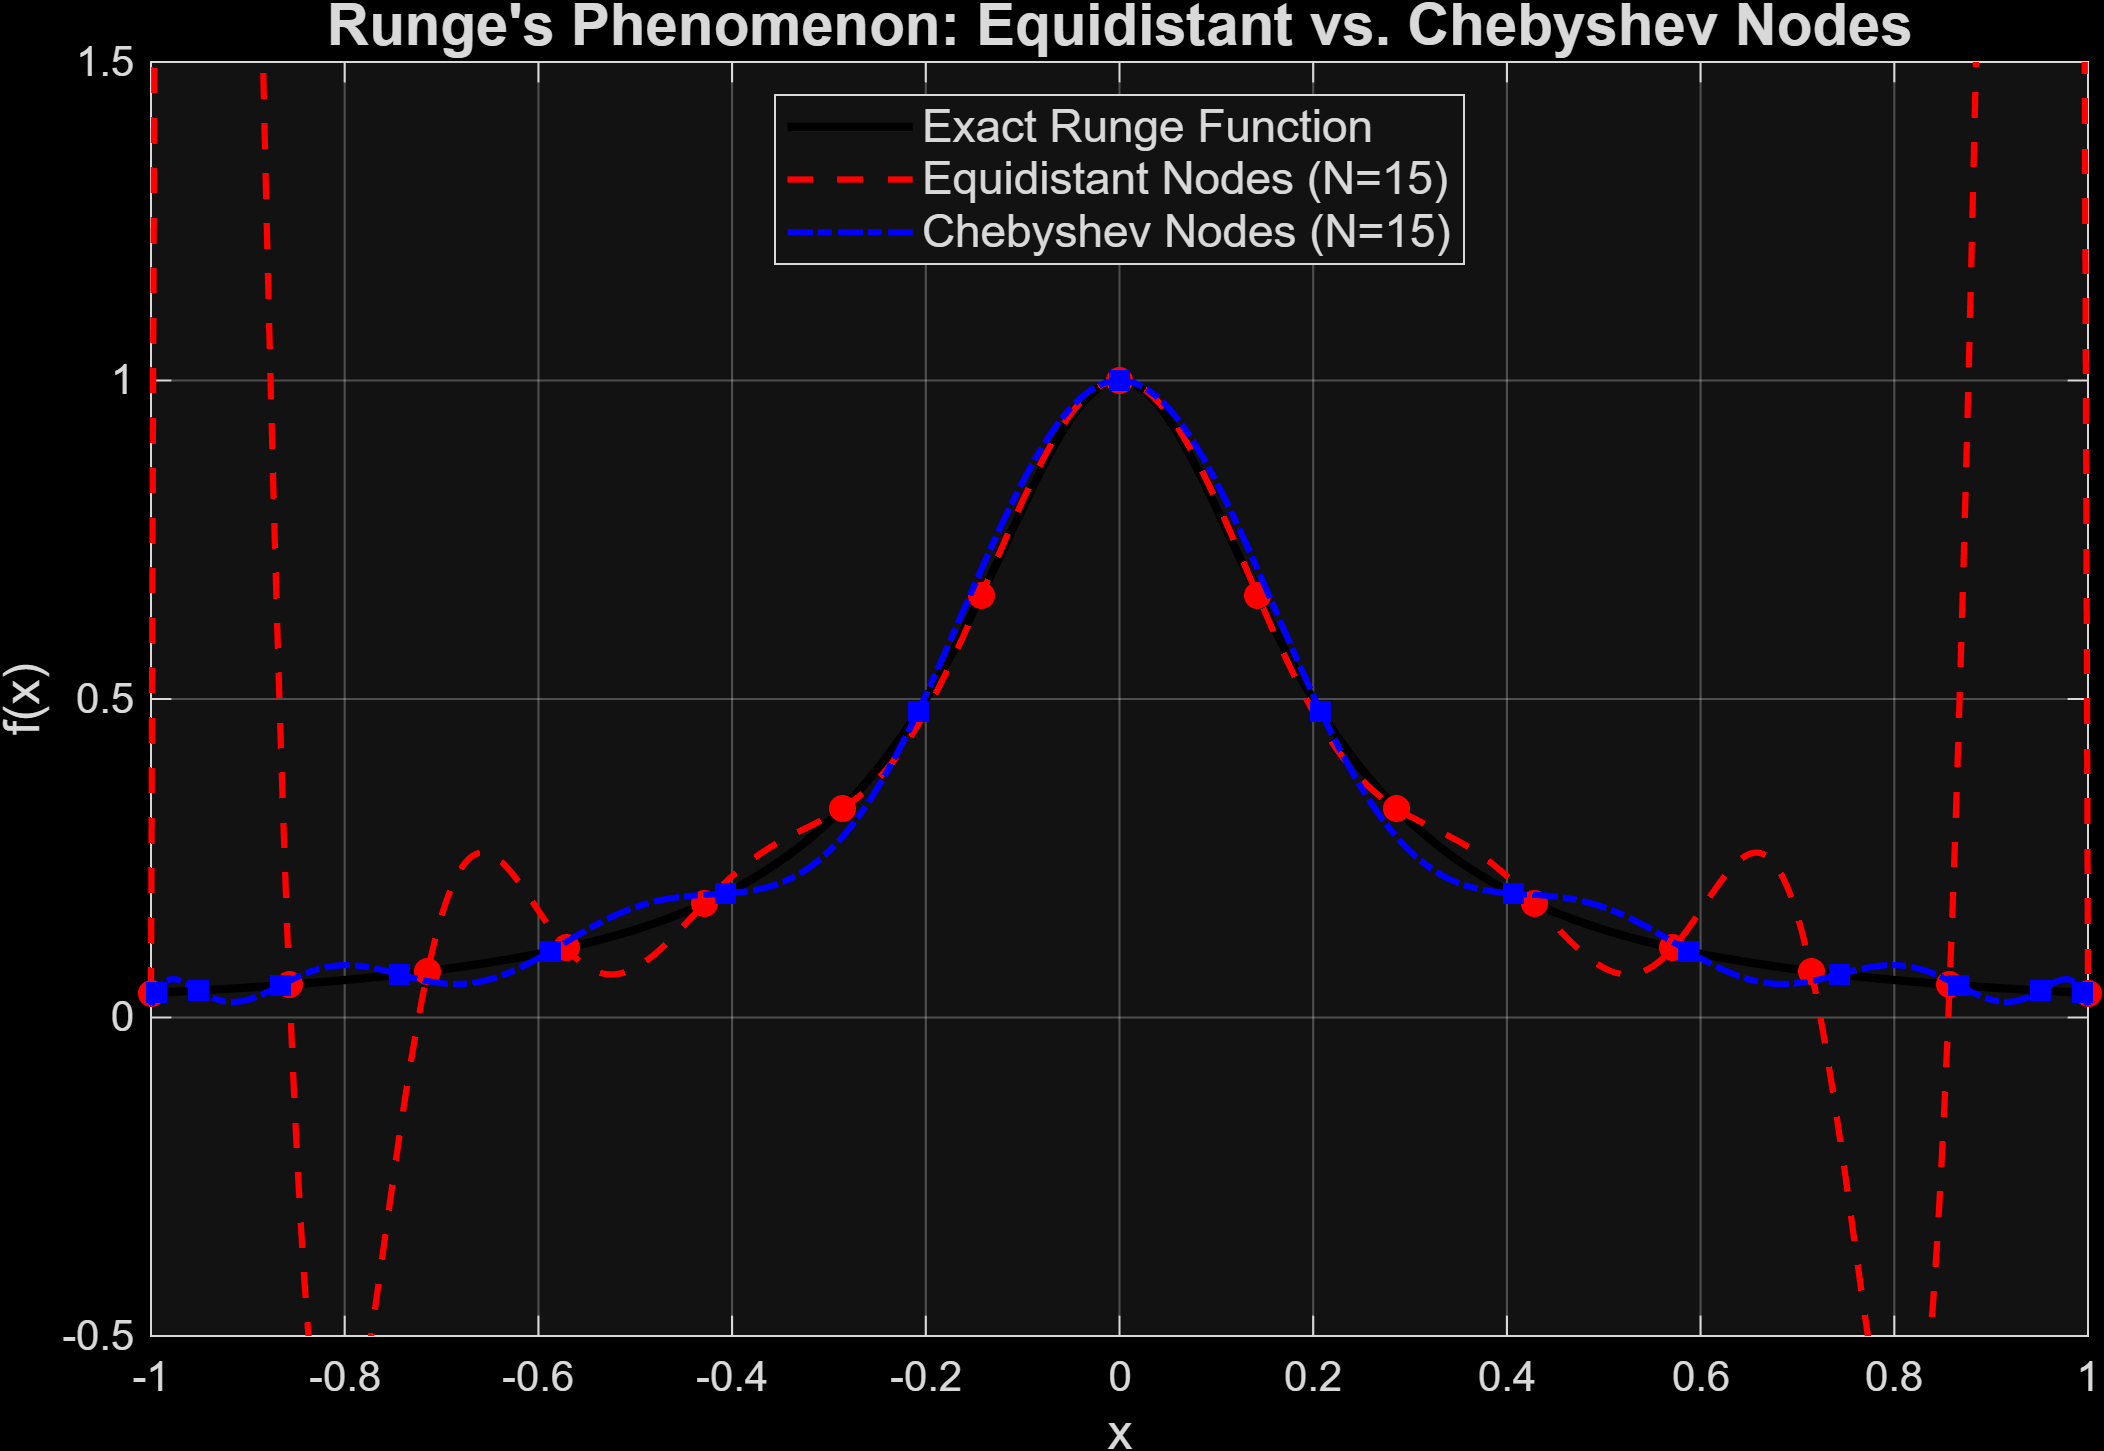
\includegraphics[width=0.8\textwidth]{runge_plot.png}
    \caption{MATLAB simulation illustrating the divergence of equidistant nodes (Runge's phenomenon) versus the stability of Chebyshev nodes.}
    \label{fig:runge}
\end{figure}

\newpage
\begin{thebibliography}{9}

\bibitem{barwolff}
Bärwolff, G.: \textit{Numerik für Ingenieure, Physiker und Informatiker}, 3. Auflage, 2006.

\bibitem{course4}
Prof. Micula Sanda, \textit{Course 4: Approximation of Functions}, Babeș-Bolyai University.

\bibitem{course5}
Prof. Micula Sanda, \textit{Course 5: Approximation of Functions}, Babeș-Bolyai University.

\bibitem{heath}
Heath, M.T.: \textit{Scientific Computing: An Introductory Survey}, International edition, 1979.

\bibitem{isaacson}
Isaacson, E., Keller, H.B.: \textit{Analysis of Numerical Methods}, Dover Edition, 1994.

\bibitem{knorrenschild}
Knorrenschild, M.: \textit{Numerische Mathematik: Eine beispielorientierte Einführung}, 5. aktualisierte Auflage, 2012.

\bibitem{runge}
Cosgun, A., Nies, J.: \textit{Exploring Runge's phenomenon}, Université du Luxembourg, 2022.

\bibitem{schatzman}
Schatzman, M.: \textit{Numerical Analysis: a mathematical introduction}, 2002.

\end{thebibliography}
\end{document}